\documentclass{report}

% cSpell:disable

% cSpell:disable

% LAYOUT --------------------------------------- 

% Page setup etc. packages
\usepackage{geometry} % For customizing page layout
\usepackage{setspace} % For setting line spacing
\usepackage{fancyhdr} % Headers, footers, page number etc.
\usepackage{textpos} % For text positioning
\usepackage{mathptmx} % Use Times New Roman font
\usepackage[T1]{fontenc} % For font encoding

\renewcommand{\headrulewidth}{0pt} % Remove header line
\fancypagestyle{plain}{ % Redefine the plain page style
\fancyhf{} % Clear footer 
}

% Set paper-size and margins
\geometry{a4paper,
hmargin = {25.4mm, 25.4mm}, % Right and left margin
vmargin = {30mm, 30mm} % Top and bottom margin
}

% Line spacing and lists
\usepackage{enumitem} % For customizing lists
\usepackage{caption} % For customizing captions

\setlist{noitemsep} % No space between list items
\setlist{nosep} % No space around list items

\captionsetup[table]{position=above, skip=5pt} % Set table captions above tables with 5pt space
\captionsetup[figure]{position=below, skip=5pt} % Set figure captions below figures with 5pt space

\onehalfspacing % Set line spacing to 1.5
\setlength{\parindent}{0pt} % No indent on new paragraphs

\pagestyle{fancy}
\fancyhf{} % Clear all header and footer fields

% Set header font to Times New Roman
\fancyhead[L]{\ifnum\value{chapter}>0\fontfamily{ptm}\selectfont Chapter \thechapter\fi} % Left header
\fancyhead[R]{\fontfamily{ptm}\selectfont \rightmark} % Right header

% Set footer
\fancyfoot[C]{\thepage} % Center footer with page number

% Ensure the header uses Times New Roman
\renewcommand{\chaptermark}[1]{\markboth{\fontfamily{ptm}\selectfont Chapter \thechapter}{}} % Chapter mark
\renewcommand{\sectionmark}[1]{\markright{\fontfamily{ptm}\selectfont \thesection\ #1}} % Section mark

% Color stuff
\usepackage[dvipsnames]{xcolor} % For color definitions
\usepackage{transparent} % For transparency in color definitions
\usepackage{soul} % For highlighting text
\usepackage[normalem]{ulem} % For underlining text while allowing underline


\definecolor{lightblue}{RGB}{247, 247, 252} % Custom color lightblue
\definecolor{lightgrey}{RGB}{247, 247, 247} % Custom color lightgrey
\definecolor{darkblue}{RGB}{41, 82, 163} % Custom color darkblue
\definecolor{brightgreen}{RGB}{82, 163, 0} % Custom color brightgreen
\definecolor{apricot}{rgb}{0.98, 0.81, 0.69} % Custom color apricot

% APPENDIX SETUP -----------------------------------
\usepackage{appendix} % For setting up appendix titles

% FONT STUFF ----------------------------------------
\usepackage{setspace} % For line spacing
\onehalfspacing % Set line spacing to 1.5

\usepackage{mathptmx} % Use Times New Roman font
\usepackage[T1]{fontenc} % For font encoding
\usepackage{titlesec} % For setting fonts on titles
\usepackage{tocloft} % For customizing TOC
\usepackage{anyfontsize} % For setting custom font sizes

\titleformat{\chapter}[display]{\Huge\bfseries\fontencoding{T1}\rmfamily\selectfont}{Chapter \thechapter}{0ex}{}[] % Set chapter font

% Set section, subsection and subsubsection fonts
\titleformat*{\section}{\fontsize{18}{21.6}\selectfont\bfseries\fontencoding{T1}\rmfamily\selectfont} 
\titleformat*{\subsection}{\fontsize{14}{16.8}\selectfont\bfseries\fontencoding{T1}\rmfamily\selectfont}
\titleformat*{\subsubsection}{\fontsize{12}{14.4}\selectfont\bfseries\fontencoding{T1}\rmfamily\selectfont}
\titleclass{\subsubsubsection}{straight}[\subsection] % Create subsubsubsection

\newcounter{subsubsubsection}[subsubsection] % This and below is for specifying the design of the subsubsubsection
\renewcommand\thesubsubsubsection{\thesubsubsection.\arabic{subsubsubsection}}
\titleformat{\subsubsubsection}
  {\normalfont\fontsize{12}{14.4}\bfseries}{\thesubsubsubsection}{1em}{}
\titlespacing*{\subsubsubsection}
{0pt}{3.25ex plus 1ex minus .2ex}{1.5ex plus .2ex}
\setcounter{secnumdepth}{4} % Allow numbering up to \subsubsubsection
\setcounter{tocdepth}{4}   % Include \subsubsubsection in the table of contents

\renewcommand{\cfttoctitlefont}{\huge\bfseries\fontencoding{T1}\rmfamily\selectfont} % Set TOC title font
  
% FIGURES AND FLOATS ---------------------------------------
\usepackage{graphicx} % Required for inserting images
\usepackage{tikz} % Required for drawing
\usepackage{tabularx} % For customizing tables
\usepackage{subcaption} % For subfigures
\usepackage{multicol} % For multiple columns
\usepackage{parcolumns} % For parallel columns
\usepackage{enumitem} % For better control over item spacing in parcolumns pckg
\usepackage{float} % For better control over float positions
\usepackage{array} % For customizing arrays
\usepackage{makecell} % For customizing cells in tables
\usepackage{multirow,bigdelim} % For multirow and bigdelim in tables
\usepackage{longtable} % For tables that span multiple pages
\usepackage[utf8]{inputenc} % For special characters in tables
\usepackage{seqsplit} % For splitting long sequences
\usepackage{eso-pic} % For adding images to title page
\usepackage[table]{xcolor} % For coloring rows in tables
\usepackage{placeins} % For controlling float positions

\usetikzlibrary{fit, backgrounds} % For fitting nodes in tikz
\usetikzlibrary{arrows,shapes,positioning,decorations.pathreplacing} % For arrows and shapes in tikz
\usetikzlibrary{decorations.pathmorphing} % For snake lines in tikz

\usepackage{caption} % For customizing captions
\captionsetup{
  labelfont=bf, % Bold label (Figure x.x, Table x.x)
  textfont=it % Italic text for the caption
}

% REFERENCING AND CITING ---------------------------------------
\usepackage[sorting=none]{biblatex} % Add sorting=none to order by citation
\usepackage{hyperref} % Hyperrefs in TOC, cites, refs etc.
\usepackage{pdfpages} % For including pdfs in the appendix
\usepackage{url} % For including urls in the .bib file (if needed for slides)


\addbibresource{references.bib}
\setcounter{tocdepth}{3}

\makeatletter % Add subsubsubsection to TOC
\newcommand{\l@subsubsubsection}{\@dottedtocline{4}{7em}{4em}}
\makeatother % Add subsubsubsection to TOC

\hypersetup{ % Set hyperref link colors
    colorlinks,
    citecolor=black,  
    filecolor=black,
    linkcolor=black,
    urlcolor=blue
    }

\urlstyle{same} % Set the URL-font to the same as the rest of the document

\renewcommand*{\bibfont}{\fontfamily{ptm}\selectfont} % Ensure bibliography is in Times New Roman

\setcounter{secnumdepth}{4} % Allow numbering up to \subsubsubsection
\setcounter{tocdepth}{4}   % Include \subsubsubsection in the table of contents

\hypersetup{ % Set hyperref link colors and bookmark depth
    colorlinks,
    citecolor=black,  
    filecolor=black,
    linkcolor=black,
    urlcolor=blue,
    bookmarksdepth=4 % Ensure bookmarks include \subsubsubsection
}

% MATH MODE PACKAGES  ---------------------------------------
\usepackage{amsmath} % For math stuff
\usepackage{amstext} % for \text macro
\usepackage{amsfonts}
\usepackage{amssymb}
\usepackage{nicematrix} % For creating nice matrices
\usepackage{booktabs} % For making tables look nice
\renewcommand{\arrayrulewidth}{0.5pt} % Set table line width

% Custom math operators
\DeclareMathOperator*{\argmax}{arg\,max}
\DeclareMathOperator*{\argmin}{arg\,min}
\DeclareMathOperator{\E}{\mathbb{E}} % blackboard E (expectation)
\DeclareMathOperator{\R}{\mathbb{R}} % blackboard R (real number)
\newcommand{\dbar}[1]{\bar{\bar{#1}}} % double bar over symbol
\newcommand{\mtext}[1]{\textbf{#1} \quad} % text before equation
\newcommand{\card}[1]{\vert #1 \vert} % cardinality sign

% CODE PACKAGES -------------------------------------
\usepackage{listings}  
\usepackage{textcomp} % special character package for making code copy-able

\definecolor{codebackground}{HTML}{f7f7f7} % background for code listings
\definecolor{codecomment}{HTML}{55aa55} % comment color for code listings
\definecolor{codekeyword}{HTML}{bc5a65} % keyword color for code listings
\definecolor{codestring}{HTML}{317ecc} % string color for code listings

% Setting up custom code style
\lstdefinestyle{codestyle}{
    language=R,
    backgroundcolor=\color{codebackground},
    basicstyle=\ttfamily, % style of base font settings
    keywordstyle=\color{codekeyword}, % style of arrows, functions etc.
    identifierstyle=, % style of variable names
    commentstyle=\color{codecomment}, % style of comments
    stringstyle=\color{codestring}, % style of strings (everything in "")
    frame=lines, % top and bottom frame (used as padding)
    framerule=5pt, % width of frame rules
    rulecolor=\color{codebackground}, % set color of frame rules
    upquote=true, % setting for making code copy-able
    columns=fullflexible % setting for making code copy-able
}

\lstset{style=codestyle} % define default code-listing style

\lstdefinestyle{outputstyle}{
    language=R,
    backgroundcolor=,
    basicstyle=\ttfamily, % style of base font settings
    keywordstyle=, % style of arrows, functions etc.
    identifierstyle=, % style of variable names
    commentstyle=, % style of comments
    stringstyle=, % style of strings (everything in "")
    frame=lines, % top and bottom frame (used as padding)
    framerule=5pt, % width of frame rules
    rulecolor=\color{white}, % set color of frame rules
    upquote=true, % setting for making code copy-able
    columns=fullflexible % setting for making code copy-able
}

% COLOR BOXES ---------------------------------------
\usepackage[theorems, many]{tcolorbox} % For creating colored boxes

%\newtcbtheorem[⟨initoptions⟩]{⟨name⟩}{⟨displayname⟩}{⟨options⟩}{⟨prefix⟩}

\newtcbtheorem[auto counter, number within=chapter]{theorem}{Theorem} % Theorem box
{colback=lightblue, % Background color
colframe=darkblue, % Frame color
coltitle=darkblue, % Title color
fonttitle=\large\bfseries\sffamily, % Title font
title=Theorem~\thetcbcounter, % Title
separator sign = \quad, % Seperator between label and title
list entry=Theorem~\thetcbcounter \quad #2, % List entry
boxrule=0.5pt, % Frame width
sharp corners, % No rounded corners
enhanced jigsaw, % Better frame drawing
detach title, % Title is not part of the box
code={\ifdefempty{\tcbtitletext}{}{\tcbset{before upper={\tcbtitle\par\medskip}}}} % Add title back
}{th}

\newtcbtheorem[auto counter, number within=chapter]{definition}{Definition} % Definition box
{colback=lightblue, % Background color
colframe=darkblue, % Frame color
coltitle=darkblue, % Title color
fonttitle=\large\bfseries\sffamily, % Title font
title=Definition~\thetcbcounter, % Title
separator sign = \quad, % Seperator between label and title
list entry=Definition~\thetcbcounter \quad #2, % List entry
boxrule=0.5pt, % Frame width
sharp corners, % No rounded corners
enhanced jigsaw, % Better frame drawing
detach title, % Title is not part of the box
code={\ifdefempty{\tcbtitletext}{}{\tcbset{before upper={\tcbtitle\par\medskip}}}} % Add title back
}{df}

\newtcbtheorem[auto counter, number within=chapter]{method}{Method} % Method box
{colback=lightblue, % Background color
colframe=black, % Frame color
coltitle=black, % Title color
fonttitle=\large\bfseries\sffamily, % Title font
title=Method~\thetcbcounter, % Title
separator sign = \quad, % Seperator between label and title
boxrule=0.5pt, % Frame width
sharp corners, % No rounded corners
enhanced jigsaw, % Better frame drawing
detach title, % Title is not part of the box
code={\ifdefempty{\tcbtitletext}{}{\tcbset{before upper={\tcbtitle\par\medskip}}}} % Add title back
}{mt}

\newtcbtheorem[auto counter, number within=chapter]{proof}{Proof} % Proof box
{colback=white, % Background color
coltitle=black, % Title color
fonttitle=\large\bfseries\sffamily, % Title font
title=Proof~\thetcbcounter, % Title
separator sign = \quad, % Seperator between label and title
borderline west={3pt}{0pt}{black}, % Left border
frame hidden, % No frame
sharp corners, % No rounded corners
enhanced jigsaw, % Better frame drawing
detach title, % Title is not part of the box
code={\ifdefempty{\tcbtitletext}{}{\tcbset{before upper={\tcbtitle\par\medskip}}}} % Add title back
}{pf}

\newtcbtheorem[auto counter, number within=chapter]{example}{Example} % Example box
{colback=white, % Background color
coltitle=brightgreen, % Title color
fonttitle=\large\bfseries\sffamily, % Title font
title=Example~\thetcbcounter, % Title
separator sign = \quad, % Seperator between label and title
borderline west={3pt}{0pt}{brightgreen}, % Left border
frame hidden, % No frame
sharp corners, % No rounded corners
enhanced jigsaw, % Better frame drawing
detach title, % Title is not part of the box
code={\ifdefempty{\tcbtitletext}{}{\tcbset{before upper={\tcbtitle\par\medskip}}}} % Add title back
}{ex}

\newtcolorbox[]{important}{ % Important box
colback=white, % Background color
coltitle=red, % Title color
fonttitle=\large\bfseries\sffamily, % Title font
title=Important, % Title
borderline west={3pt}{0pt}{red}, % Left border
frame hidden, % No frame
sharp corners, % No rounded corners
enhanced jigsaw, % Better frame drawing
}

\newtcolorbox[]{highlight}{ % Highlight box
colback=white, % Background color
coltitle=darkblue, % Title color
fonttitle=\large\bfseries\sffamily, % Title font
borderline west={3pt}{0pt}{darkblue}, % Left border
frame hidden, % No frame
sharp corners, % No rounded corners
enhanced jigsaw, % Better frame drawing
}

% OTHER ---------------------------------------
\usepackage[style=ddmmyyyy]{datetime2} % Generates todays date 
\usepackage{lipsum} % Generates lorem ipsum text
\usepackage{chemfig} % For drawing chemical structures


% Add this line to your preamble, replace "references.bib" with the name of your .bib file
\addbibresource{references.bib}

\begin{document}

\begin{titlepage}

    \TPGrid{12}{24}
    
    \begin{textblock}{9.4}(0,7.5)
        \Huge{\fontfamily{ptm}\selectfont\bfseries{Fruit and Berry Crop Physiology and }}
    \end{textblock}
    \begin{textblock}{9.4}(0,8.5)
        \Huge{\fontfamily{ptm}\selectfont\bfseries{Quality}}
    \end{textblock}
    \begin{textblock}{9.4}(0,9.5)
        \Huge{\fontfamily{ptm}\selectfont\bfseries{NPLK14014U}}
    \end{textblock}
    
    \begin{textblock}{9.4}(0,10.5)
        \LARGE{\fontfamily{ptm}\selectfont\bfseries{Notes taken during the course, including lectures, exercises, curriculum, and practicals}}
    \end{textblock}
    
    \begin{textblock}{9.4}(0,13)
        \large{\fontfamily{ptm}\selectfont\bfseries{
        Lucas Daniel Paz Zuleta, TZS159}}
    \end{textblock}
    
    \begin{textblock}{9.4}(0,13.5)
        \large{\fontfamily{ptm}\selectfont{MSc student at the University of Copenhagen}}
    \end{textblock}
    
    \begin{textblock}{9.4}(0,16)
        \large{\fontfamily{ptm}\selectfont{Last compiled: \today}}
    \end{textblock}
    
    \begin{textblock}{8.4}(0,16.5)
        \large{\fontfamily{ptm}\href{https://github.com/DanishUnicorn/tcp}{Link to GitHub reporsitory}}
    \end{textblock}
    
    \AddToShipoutPicture*{\put(-10, 45){\includegraphics*[width=20cm]{KU_titelpage/logos/science-english.pdf}}} % KU text
    
    \AddToShipoutPicture*{\put(0, 45){\includegraphics*[width=21cm]{KU_titelpage/logos/ku-logo.pdf}}} % KU logo
    
    \AddToShipoutPicture*{\put(482, 0){\includegraphics*[width=4cm]{KU_titelpage/logos/dk_uni.pdf}}} % dk_unicorn_temp logo
    
    \end{titlepage} % Insert frontpage file.

\pagenumbering{gobble} % Turn off page numbering
\addtocontents{toc}{\protect\setcounter{tocdepth}{-1}} % Temporarily disable TOC entries
\chapter*{Course Description}
\setlength{\headheight}{12.71342pt}
\addtolength{\topmargin}{-0.71342pt}

\section*{Education}
MSc Programme in Agriculture


\section*{Content}
The focus is on fruit growth and fruit quality in relation to the use as fresh fruits or for processing. How is fruit growth and quality affected by the plants' physiological and genetic basis and how can it be influenced by different growing techniques and environmental factors? Similarities and differences among the fruit crop types (pit fruits, stone fruits, berries and nuts), with regard to demands in growing conditions are discussed. Furthermore, we analyze which physiological parameters are important in the different fruit species for determining yield and important quality components. Emphasis is on temperate fruits, nuts, berries and fruit vegetables, grown mainly in open field or in tunnel systems. The reference growing systems are the common commercial systems, including organic growing. The course also addresses examples of the genetic and quality variation among cultivars and the importance of different quality attributes in relation to postharvest use (fresh consumption, cooking, juice processing or fruit wine making).
In general the crop specific aspects of the following main topics will be covered:
\begin{itemize}
    \item Yield and quality components (organ development and interactions) and determinant factors
    \item Allocation of dry matter and nutrient  among sources and sinks in fruiting plants
    \item Control of vigour and plant structure by pruning and management of nutrients and irrigation
    \item Effects of preharvest factors (climate, a-biotic or biotic stresses) on internal and external quality of fruits
    \item Content and development of secondary and bioactive compounds in fruits.
    \item Maturation, ripening and assessment of optimal harvest and quality aspects of fruits and berries.
    \item Post harvest usability and sensory aspects of different cultivars and fruit types.
\end{itemize}  

In addition to fresh use,  special attention is given to production and quality of fruit juices.
Biotechnological aspects are addressed at a limited level.


\section*{Learning Outcome}
The course is targeted to students interested in plant science (Horticulture and Agriculture) and food science students who are particularly interested in fruit and berry crops and the quality and use of the raw materials/food products these crops provide.
\subsection*{Knowledge}

\begin{itemize}
    \item The physiological basis for production of fruiting crops (including fruit vegetables such as tomato and cucumber).
    \item Overview of development of the major plant organs with focus on the fruit and its quality and understand how and why it varies with genotype and preharvest growing conditions
    \item Describe the variation among the major cultivars used of fruits and berries in terms of development and quality parameters.
    \item Reflect on the importance of fruit and berries for human health
\end{itemize}

\subsection*{Skills}

\begin{itemize}
    \item Apply basic knowledge of physiology and biochemistry from plant and food science at the whole plant and organ level.
    \item Analyse a fruiting crop based on the crop specific yield and quality components.
    \item Explain how and why different techniques are used in the fruit industry and how it affects plant growth and product/fruit quality.
\end{itemize}

\subsection*{Competences}

\begin{itemize}
    \item Analyse the methods used to obtain optimal productivity and product quality.
    \item Discuss trade offs in management, such as between optimal sensory quality and storability, between yield and quality or pesticide use vs organic growing
\end{itemize}


\section*{Litterature}
Literature lists will be available from the course responsible.


\section*{Recommended Academic Qualifications}
Academic qualifications equivalent to a BSc degree is recommended.


\section*{Teaching and Learning Methods}
Besides lectures the course will include practicals, where the students are working with cultivar evaluation, quality analysis or aspects of fruit growing physiology (plant and organ development etc). Part of the hands on teaching will be field based in the experimental fruit collections at the Pometum.

\vspace*{1em}
The practicals will be made in groups, while the individual student is given the opportunity, in a major report written throughout the course, to focus on an area of special interests. Thus individual competences with emphasis on either fruit growing physiology or fruit quality aspects of fruits as raw materials for industry processing or fresh consumption can be developed. The topic of the major report are to be presented to the class in a short lecture based on a selected journal paper.
\vspace*{1em}

2 or 3 excursions will be arranged in connection with the different course subjects.

\section*{Workload}

\begin{table}[h]
    \centering
    \caption{A table with an overview over the workload for the course.}
    \label{tab:workload}
    \rowcolors{2}{white}{gray!7}
    \begin{tabular}{ l | c}
        \textbf{Category} & \textbf{Hours} \\ 
        \hline
        Lectures & 35 \\ 

        Class Instruction & 5 \\

        Preparation & 40 \\ 

        Practical exercises & 30 \\

        Excursions & 21 \\

        Project work & 75 \\

        \hline
        Total & 206 \\ 
    \end{tabular}
\end{table}

\section*{Exam}

\begin{table}[h]
    \centering
    \caption{A table with an overview over the elaborated description of the course}
    \label{tab:elaborated_description}
    \rowcolors{2}{white}{gray!7}
    \begin{tabular}{ l | p{10cm} }
        Credit & 7.5 ECTS \\ 
        
        Type of assessment & \begin{itemize}
                                \item Oral examination, 20 minutter
                                \item Written assignment, ca. 3 uger
                            \end{itemize} \\ 

        Type of assessment details & The portfolio includes a major report and 2 out of 4 additional products (e.g. exercise reports or presentation)

        Weight of exam components: Evaluation of major report 50 \%, oral examination in portfolio contents and curriculum 50\%. \\

        Examination prerequisites & Submitted and approval of the reports for theoretical and practical exercises \\ 

        Aid & All aids allowed 

        \href{https://kunet.ku.dk/study/food-science-technology-ma/Pages/topic.aspx?topicid=20fc0507-633c-455d-85ae-eb53a44d4072}{Read about how to use Generative AI on KuNet}\\

        Marking scale & 7-point grading scale \\

        Censorship form &   \begin{itemize}
                                \item No external censorship
                                \item One internal examiner
                            \end{itemize} \\

        Re-exam &   The exam is an oral exam, as for the ordinary exam. Submission of an individual major report 1 week before the oral re-exam is required. The topic may be as for the ordinary exam but in a revised version. \\ 
    \end{tabular}
\end{table}


\newpage
\addtocontents{toc}{\protect\setcounter{tocdepth}{4}} % Re-enable TOC entries
\tableofcontents
\clearpage % ends the page, to ensure page numbering starts on the next page where the main text begins

\pagestyle{fancy}
\fancyfoot{} % Clear footer
\fancyhead[R]{\sffamily\thepage} % Set page number in header
\fancyhead[L]{{\bfseries\sffamily Chapter \thechapter \, |} \quad {\transparent{0.6}\sffamily\rightmark}} % Set chapter name in header

\pagenumbering{arabic} % Turn on page numbering

\setcounter{chapter}{1} % Set chapter number to 1
\renewcommand{\thesection}{\arabic{section}} % Customize section numbering to be just "1", "2", etc.
% Start the main content of the document
\setcounter{chapter}{0}
\setcounter{section}{0}
\chapter{Lecture Notes}
\setlength{\headheight}{12.71342pt}
\addtolength{\topmargin}{-0.71342pt}

\section{Lecture 01 - 02/09-2025}
\subsection{The Tropical Environment} 

\subsubsection{Aim} 
\begin{itemize} 
    \item Overview the most important aspects of tropical climates. 
    \item Ability to figure out how the climate is likely to be in certain places in the tropics. 
    \item Idea of which crop you can grow. 
\end{itemize}

\subsection{What Determines the Climate?} 
The climate is determined by several factors, including temperature and precipitation. Key aspects are the yearly average temperature and the yearly range in temperature, as some areas experience a larger difference between the highest and lowest temperatures than others. Similarly, average precipitation is important, but the yearly variation in rainfall also plays a significant role.
\subsubsection*{Core takeaway:} 
Climate is primarily defined by temperature and precipitation, considering both yearly averages and seasonal variations. Likely exam-relevant.

\subsection{Classification: Latitudes} 

\begin{itemize} 
    \item Tropical zone from 0\textdegree–23.5\textdegree (between the tropics) latitude: Here, solar radiation reaches the ground nearly vertically, more water evaporates, and the air is often moist. A dense cloud cover reduces the effect of solar radiation on ground temperature. 
    \item Subtropics from 23.5\textdegree–40\textdegree latitude: These regions receive the highest radiation in summer, have relatively thin cloud cover, and receive less moisture. 
    \item Temperate zone from 40\textdegree–60\textdegree latitude: This zone is characterized by significantly differing seasons and day lengths, less frequent climate extremes, a more regular distribution of precipitation, and a longer vegetation period. 
    \item Cold zone from 60\textdegree–90\textdegree latitude: The poles in this zone receive less heat through solar radiation, and day length varies the most. Vegetation is only possible during a few months and is often sparse. 
\end{itemize}

\subsubsection*{Core takeaway:} 
Earth's climate zones are classified by latitude, each with distinct characteristics regarding solar radiation, temperature, precipitation, and vegetation periods. Likely exam-relevant.


\subsection{Circles of Latitude and Longitude} 
\subsubsection{Earth's Movement and Tropical Rain Belt} 
The Earth spins around its axis, akin to a top, a process known as Earth's rotation. Simultaneously, it orbits or revolves around the Sun. The tropical rain belt runs along the equator and extends to about the Tropic of Cancer (23.5\textdegree north latitude) and Tropic of Capricorn (23.5\textdegree south latitude). By approximately 30\textdegree north and south latitude, the air cools enough to sink back to the surface, creating high pressure (H) and drier conditions.
\subsubsection{Earth's Orbit and Solar Energy} The Earth's revolution around the sun takes 365.24 days. At the equator, the Earth rotates at roughly 1,700 km per hour. The Earth is closest to the sun (perihelion) on January 3rd at 147 million km, moving faster at 27 km/s. It is furthest from the sun (aphelion) on July 4th at 152 million km, moving slower. Solar energy is relatively constant, approximately 400 W/m$^2$/year. About 300 W/m$^2$/year is lost as terrestrial re-radiation, leaving a surplus of 100 W/m$^2$ at the surface. Most of the radiation is absorbed by the Earth and warms it. Some of the outgoing infrared radiation is trapped by the Earth’s atmosphere, which also contributes to warming.

\subsubsection*{Core takeaway: }
Earth's rotation and revolution influence climate patterns, including the tropical rain belt, and its interaction with solar energy dictates global temperatures. Likely exam-relevant. 


\subsection{The Tropics} 
The tropics are characterized by a high input of solar radiation and high maximum temperatures, with little variation in temperature. Water supply is the most significant variable, marked by high rainfall variability and high rainfall intensity. The tropics cover 42\% of the Earth's surface. 
\subsubsection{Characterize the tropics !} 
\subsubsection{Precipitation} 
Precipitation patterns in the tropics include: 
\begin{itemize} 
    \item Wet climate (between 5\textdegree and 10\textdegree of the equator). 
    \item Wet dry climate (between 10\textdegree and 20\textdegree). 
    \item Two wet seasons: typically 1000-2000 mm (e.g., Salvador, Abidjan). 
    \item Two shorter rainy seasons (e.g., Nairobi). 
    \item One long rainy season: monsoonal, 750-1500 mm (e.g., Manila). 
    \item One short rain season: 250-750 mm (e.g., Darwin, Hyderabad). 
    \item Dry climate (e.g., Alice Springs, Lima, Khartoum)
\end{itemize}


\subsubsection*{Core takeaway:} 
The tropics receive high solar radiation and experience consistent high temperatures, with water supply and significant rainfall variability being defining features across different precipitation zones. Likely exam-relevant.


\subsection{Three Major Biomes} 
A biome is defined as a community of similar plants and animals occupying a large area. The three major biomes are Forest, Savanna, and Desert. 

\subsubsection{Tropical biomes and annual precipitation (mm)} Tropical biomes exhibit extremely high biodiversity, encompassing 50\% of the world’s terrestrial plant and animal species, despite covering only about 6\% of the world’s land area.

\subsubsection*{Core takeaway:} 
The tropics host three major biomes—Forest, Savanna, and Desert—which are critical for global biodiversity, harboring half of the world's terrestrial species in a small land area. Likely exam-relevant.


\subsection{Deforestation} 
Before human intervention, rainforests covered 15\% of the Earth's land area, but today they cover only 6\%. In the last 200 years, the total area of rainforest has decreased from 1,500 million hectares to less than 800 million hectares. A third of tropical rainforests have been destroyed in just the last 50 years. Approximately 119,000 - 150,219 km$^2$ are lost each year, affecting the world's most spectacular ecosystems.

\subsubsection*{Core takeaway: }
Deforestation has drastically reduced tropical rainforest coverage, leading to a significant loss of these vital ecosystems globally. Likely exam-relevant.


\subsection{Daily Weather Cycle in the Tropical Rainforest} 
In the morning, the sun shines and heats up the ground, causing hot and wet air to rise. In the afternoon, dark clouds form, bringing rain and thunderstorms to the rainforest.


\subsection{Prevailing Winds} 
\subsubsection{Latitudinal Variation in Evapotranspiration and Precipitation} 
(figure, see slide 9)
\subsection{Remember!} 
\begin{itemize} 
    \item Hot air weighs less than cold air. 
    \item Hot air can contain more water than cold air. 
    \item Air will flow from areas of high pressure towards areas with low pressure. 
    \item Condensation of water releases energy. 
    \item The temperature of the air drops approximately 1 degree for every 100 m, or 0.5 degrees if the air contains water. 
    \item Objects moving in the northerly or southerly direction will be deflected clockwise in the northern hemisphere and counter-clockwise in the southern hemisphere (Coriolis force) (see also Slide 10). 
\end{itemize}

\subsubsection*{Core takeaway:} 
Atmospheric dynamics, driven by temperature, pressure, and the Coriolis force, dictate air movement, moisture content, and temperature changes critical for understanding weather patterns. Likely exam-relevant.


\subsection{Coriolis Force} 
When the Earth rotates, a point close to the equator moves much faster than a point at one of the poles. This movement creates specific patterns on Earth and affects winds and ocean currents.

\subsubsection*{Core takeaway: }
The Coriolis force, a result of Earth's rotation, deflects moving objects and significantly influences global wind and ocean current patterns. Likely exam-relevant.


\subsection{Tropical Storms} 
Tropical storms include Hurricanes (in the Caribbean and United States) and Typhoons (in the Pacific Ocean). These storms are characterized by wind speeds exceeding 115 km/hour, low pressure, and a circular pattern of isobars with a diameter of 150-650 km. They bring extreme rainfall (up to 200 mm/day) and steep gradients that produce high wind speeds. 

\subsubsection{Cyclones Around Australia}
\subsection{Monsoons} 
Monsoons are large-scale sea breezes that occur when the temperature on land is significantly warmer or cooler than the temperature of the ocean. These temperature imbalances happen because oceans and land absorb heat in different ways.

\subsubsection*{Core takeaway:} 
Tropical storms like hurricanes and typhoons are intense low-pressure systems with high winds and extreme rainfall, while monsoons are seasonal wind shifts caused by differential heating of land and sea. Likely exam-relevant.


\subsection{Southeast Asian Rainforests} 
Southeast Asian rainforests experience four different seasons: the winter northeast monsoon, the summer southwest monsoon, and two inter-monsoon seasons. 

\begin{itemize} 
    \item The northeast monsoon season (November to March) has steady winds from the north or northeast, originating from Siberia, which bring typhoons and other severe weather. The east coasts of the Southeast Asian islands receive heavy rains during this time. 
    \item The southwest monsoon season (May to September) has less wind and is slightly drier, though it still rains every day. 
    \item During the inter-monsoon seasons, the winds are light. All seasons are hot and humid, with very little seasonal variation in temperature. 
\end{itemize}

\subsubsection*{Core takeaway:} 
Southeast Asian rainforests experience distinct monsoon seasons driven by regional wind patterns, resulting in varied rainfall but consistently hot and humid conditions year-round. Likely exam-relevant.


\subsection{Tropical Rainforests} 
Tropical rainforests are characterized by a type of tropical climate with no dry season, meaning all months have an average precipitation value of at least 60 mm (2.4 in). There are no distinct summer or winter seasons; it is typically hot and wet throughout the year, with both heavy and frequent rainfall. Around the equator, there are two seasons with heavy rainfall, receiving up to 10 meters a year. As one moves away from the equator, it becomes a bit drier in some months, but there is still more than 2 meters of rain annually. Most of the rainfall does not reach the ground directly, as the trees act as a canopy and catch the rain. 

\subsubsection{Rainforest Burned Down in South America} (image, see slide 14)
\subsubsection*{Core takeaway:} 
Tropical rainforests are defined by continuous high rainfall, consistent high temperatures year-round, and the significant role of their dense canopy in intercepting precipitation. Likely exam-relevant.


\subsection{Tropical Desert} Major tropical desert areas include the Sahara and Kalahari deserts in Africa, Arabian, Iranian and Thar Deserts in Asia, Arizona and Mexican deserts in North America, and the Great Australian Desert. 

\subsubsection{Oasis with Date Palm} (image, see slide 15) 

\subsubsection{External Resources / Ecosystem Map} 
\textit{[Requires further research: This section primarily provides links to external resources (YouTube and a NOAA ecosystem map) and does not contain descriptive content within the slides themselves.]}

\subsection{A Simple Illustration of the Major Crop Types in Relation to Climate} 
\textit{[Requires further research: This slide title suggests an illustration but the content is not provided.]}

\subsubsection*{Core takeaway:} 
Tropical deserts are extensive arid regions found across multiple continents, characterized by very low precipitation and extreme temperatures. Likely exam-relevant.
%\chapter{Lecture Exercises}
\setlength{\headheight}{22.94003pt}
\addtolength{\topmargin}{-10.22661pt}




\section{Lecture 02 TE}
\subsection*{How to increase soil fertility of degraded soils?}

\begin{itemize}
    \item In this exercise we will discuss possible ways to improve the fertility of degraded soils. We discuss different options in groups. After the group discussions we will discuss in plenum.
    \item Your inputs for the discussion counts as the deliverable of the exercise.
    \item Potential Management Options to increase SOM:
    \begin{enumerate}
        \item Integration of legumes as intercrops or in rotation
        \item Inorganic fertilizer
        \item Manure (livestock)
        \item Green manure, mulching, residue retention
        \item Agroforestry techniques (including fallowing)
        \item No tillage
    \end{enumerate}
\end{itemize}

\subsection*{Questions:}
\begin{enumerate}
    \item What are the benefits of the option?
    \item Which problems could (potentially) limit the adoption?
    \item What are possible solutions to the problems/limitations?
\end{enumerate}


\chapter{Literature résumés}
\setlength{\headheight}{12.71342pt}
\addtolength{\topmargin}{-0.71342pt}

This section of the course notes is designed to streamline access to the key findings from each reading material (RM), providing a concise and accessible overview of essential information. Created through experimentation with various AI platforms, this chapter also serves to enhance prompt engineering skills, exploring diverse methods of note-taking for maximum efficiency and clarity. The procedures for creating these summaries have varied, but all methods share a common approach: each RM has been fully read, with summaries and notes prepared after completing each respective subsection. By using these AI-co-op'ed approaches, these notes aim to be both a reliable reference and a resource for continuous improvement in capturing complex microbiology concepts.

\section{1\texorpdfstring{\textsuperscript{st}}{st} Reading Material from the Curriculum}

\subsection{Milk for Liquid Consumption}
Liquid milk is treated by pasteurization or sterilization to ensure safety, extend shelf life, and retain flavour. Raw milk is considered unsafe and is restricted in many countries. Pasteurized milk retains better flavour, while sterilized milk offers longer shelf life, especially valued in cooking. Fat content is usually standardized, but low-fat and skim milks are also common. Some products are fortified or processed via ultrafiltration for consistent protein content, although this may be legally restricted. Quality attributes vary by use, and packaging is essential for hygiene \cite*{curr_rm_01_dairy_science_technology}.

\subsubsection*{Manufacture}
Thermalization reduces lipase activity and psychrotrophic growth, aiding shelf life. Homogenization prevents creaming but increases lipolysis risk, requiring higher heat (e.g., 20 s at 75~\textdegree C). Low pasteurization (15 s at 72~\textdegree C) kills pathogens while preserving natural inhibitors, though heat-sensitive compounds like agglutinins and immunoglobulins are degraded in high-pasteurized milk. Packaging hygiene is crucial to prevent recontamination and preserve shelf life \cite*{curr_rm_01_dairy_science_technology}.


\subsubsection*{Shel Life}
Shelf life is influenced by bacterial growth, enzymatic activity, and chemical/physical changes. Key factors include storage temperature, recontamination, and Bacillus cereus spore levels. Below 7~\textdegree C, psychrotrophs dominate spoilage. Hygiene in packaging is essential; rapid tests help detect recontamination \cite*{curr_rm_01_dairy_science_technology}.

\subsubsection*{Extended-Shelf-Life Milk}
ESL milk combines long shelf life with near-fresh flavour. One method applies short-time direct UHT treatment (e.g., 2 s at 140~\textdegree C) with aseptic packaging; enzymes like plasmin may still affect taste after weeks. The second method involves microbial removal via microfiltration or bactofugation, often followed by partial UHT sterilization of retentate and cream. Aseptic packaging is essential. Cooked flavour is minimized by limiting heat to fat-rich fractions \cite*{curr_rm_01_dairy_science_technology}. 

\subsection{Sterilized Milk}
\subsubsection{Description}
Sterilized milk must be microbe-free, shelf-stable at ambient temperature, and retain acceptable flavour and nutritional value. UHT sterilization (e.g., 1 s at 145~\textdegree C) minimizes browning, off-flavours, and vitamin loss. To prevent spoilage, packaging must be aseptic, and milk free from heat-resistant enzymes. Homogenization avoids creaming and coalescence. Lactulose content is used to identify UHT-treated milk \cite*{curr_rm_01_dairy_science_technology}.

\subsubsection*{Manufacture}
Sterilized milk is made via in-bottle, mild in-bottle, or flow-through UHT processes. Psychrotroph enzymes (esp. from \textit{Pseudomonas}) are heat-resistant, so raw milk must be fresh. UHT heating (>140~\textdegree C) ensures safety but risks casein aggregation, off-flavors, and vitamin loss. Aseptic homogenization and deaeration are crucial to prevent oxidized flavor. Oxygen- and light-tight packaging prolongs shelf life \cite*{curr_rm_01_dairy_science_technology}. 

\subsubsection*{Shelf Life}
Spoilage of in-bottle sterilized milk may result from surviving spores (e.g., \textit{B. subtilis}, \textit{B. stearothermophilus}) or leaky packaging. UHT milk mainly deteriorates via recontamination or residual heat-resistant enzymes, causing gelation, off-flavors, or plasmin-induced bitterness. Nonenzymatic spoilage includes oxidation, Maillard reactions, and light effects. Shelf life is tested via incubation, oxygen pressure, or ATP bioluminescence \cite*{curr_rm_01_dairy_science_technology}.

\subsection{Reconstituted Milk}
Reconstituted milk is made by dissolving milk powder in water; recombined milk adds anhydrous milk fat to reconstituted skim milk. It mimics whole milk but lacks natural fat globule membrane components. Filled milk uses vegetable oil instead of milk fat. Toned milk blends buffalo milk with skim milk to reduce fat content \cite*{curr_rm_01_dairy_science_technology}. 

\subsection{Flavour}
Good flavour means a bland taste without off-flavours. Sources include microbial growth (e.g., \textit{B. cereus}, \textit{P. fragii}), plasmin, lipoprotein lipase, and oxidation by Cu or light. Heat causes cooked, UHT ketone, or sterilized-milk flavour, depending on thermal load. Sunlight flavour arises from methionine oxidation with riboflavin present \cite*{curr_rm_01_dairy_science_technology}.

\subsection{Nutritive Value}
This section addresses changes in nutritive value due to deliberate changes in composition, processing, and storage. For details on the nutritive aspects of milk components, see Subsections 2.1.2, 2.2.4, 2.3.3, 2.4.5, and Table 2.18 in the book \cite*{curr_rm_01_dairy_science_technology}.

\subsubsection*{Modification of Composition}
Milk of modified composition includes low-fat, skim, or vitamin-fortified types. Filled milk uses vegetable oils, often rich in vitamins D and E, with added antioxidants. Calcium may be added as lactate or whey permeate. Lactose-free milk, produced by adding lactase after UHT treatment, has limited success due to cost and sweet taste. Functional foods and specialised products are also being developed \cite*{curr_rm_01_dairy_science_technology}.

\subsubsection*{Loss of Nutrients}
Pasteurized and UHT-sterilized milk lose few nutrients, while in-bottle sterilized milk shows greater loss, especially of lysine and vitamins due to Maillard reactions. Losses mainly affect vitamin C and B vitamins ($B_1$, $B_2$, $B_6$, $B_9$, $B_12$). Oxygen and light accelerate degradation, with riboflavin acting as a catalyst. Packaging permeability is crucial to prevent losses \cite*{curr_rm_01_dairy_science_technology}.

\subsection{Infant Formulas}
Breast feeding is preferable, but when not possible, infant formulas based on cows' milk fractions are used. Unmodified cows' milk is unsuitable. Due to higher risk of microbial contamination, strict hygiene is essential during preparation and storage. Liquid formulas should be refrigerated \cite*{curr_rm_01_dairy_science_technology}.

\subsubsection*{Human Milk}
Human milk differs from cows’ milk in composition and varies by individual and lactation stage. It contains more essential fatty acids, cholesterol, and oligosaccharides, but less protein, casein, and minerals. It includes immunoglobulin A, lysozyme, and lactoferrin, and lacks $\beta$-lactoglobulin. Infant formulas require significant adjustment to mimic its properties \cite*{curr_rm_01_dairy_science_technology}.

\subsubsection*{Formula Composition and Manufacture}
Infant formulas use skim milk and sweet whey (e.g., 1:5 ratio), often with added lactose, vegetable oils, vitamins, Fe, and Cu. Whey is partly desalted. Oligosaccharides or lactulose may be added. Manufacture involves wet mixing, pre-emulsification, pasteurization, and homogenization. Products may be UHT-sterilized, canned, or spray-dried \cite*{curr_rm_01_dairy_science_technology}.



%\chapter{Exam Questions and Answers}
\setlength{\headheight}{12.71342pt}
\addtolength{\topmargin}{-0.71342pt}

This chapter of the course notes compiles the exam questions for the course held in November 2025, along with their respective answers prepared by me. The purpose of this section is twofold: firstly, to provide a reflective exercise that consolidates understanding of the course material; and secondly, to document my comprehension of the course topics as assessed through the exam questions.

\vspace{1em}
To ensure citation accuracy and academic transparency, NotebookLM has been employed as the primary generative AI platform. Its use has focused on verifying that all citations accurately reference the uploaded course materials and lecture slides provided by the professors. Beyond citation control, this section also represents an ongoing exploration of prompt engineering — refining interaction design to optimise AI output quality, precision, and academic reliability. Through this approach, the work aims to maintain a high academic standard while enhancing clarity, structure, and depth in written responses.

\vspace{1em}
There are a total of 17 questions in the exam, each comprising between three and five sub-questions. The numbering of the sections in this chapter corresponds directly to the numbering of the exam questions, ensuring a clear and consistent structure throughout. Each question is presented below, followed by its respective sub-questions and answers.

\section{1: Yield and quality determinants and components}
\textbf{Shoot and bud development, growth and flower bud development}

\subsection{Characterise the development and importance of spurs and extension 
(long) shoots}
\subsection{Describe differences in bud development and structure between stone 
and pome fruits}
\subsection{Describe some important yield components in strawberry and in sour 
cherry}
\subsection{Describe some conditions which may affect the development of 
flower buds negatively}


\section{Yield and quality determinants and components}
\textbf{Flowers, pollination and fruit set (sterility and fertility)}

\subsection{Describe important factors determining fruit set? }
\subsection{What is the importance of EPP?}
\subsection{What are important quality parameters for pollen and flowers?}
\subsection{Why and how do we use pollinators?}
\subsection{Are insects (fx bees) needed in pollination of self-pollinating crops?}



%\chapter{Abbreviations and Explanations}
\setlength{\headheight}{12.71342pt}
\addtolength{\topmargin}{-0.71342pt}


\begin{longtable}{| p{5cm} | p{2cm} | p{7.5cm} |}
    \hline
    \textbf{Topic} & \textbf{Abb.} & \textbf{Description} \\ 
    \hline
    \endfirsthead
    
    \hline
    \textbf{Topic} & \textbf{Abb.} & \textbf{Description} \\ 
    \hline
    \endhead
    
    \hline \multicolumn{3}{r}{\textit{Continued on next page}} \\ 
    \endfoot
    
    \hline
    \endlastfoot
    
    \textbf{16S ribosomal RNA} & \textbf{16S rRNA} & \textit{A component of the 30S subunit of prokaryotic ribosomes, commonly used in phylogenetic studies to identify bacteria and archaea.} \\
    \hline
    \end{longtable}




\printbibliography

\begin{appendices}
    \chapter*{Appendices}
\addcontentsline{toc}{chapter}{Appendices} % This adds it to the table of contents, even though we are excluding the chapter function above.

\section{Appendix 1 - Practical Exercise 01}
\label{appendix1}
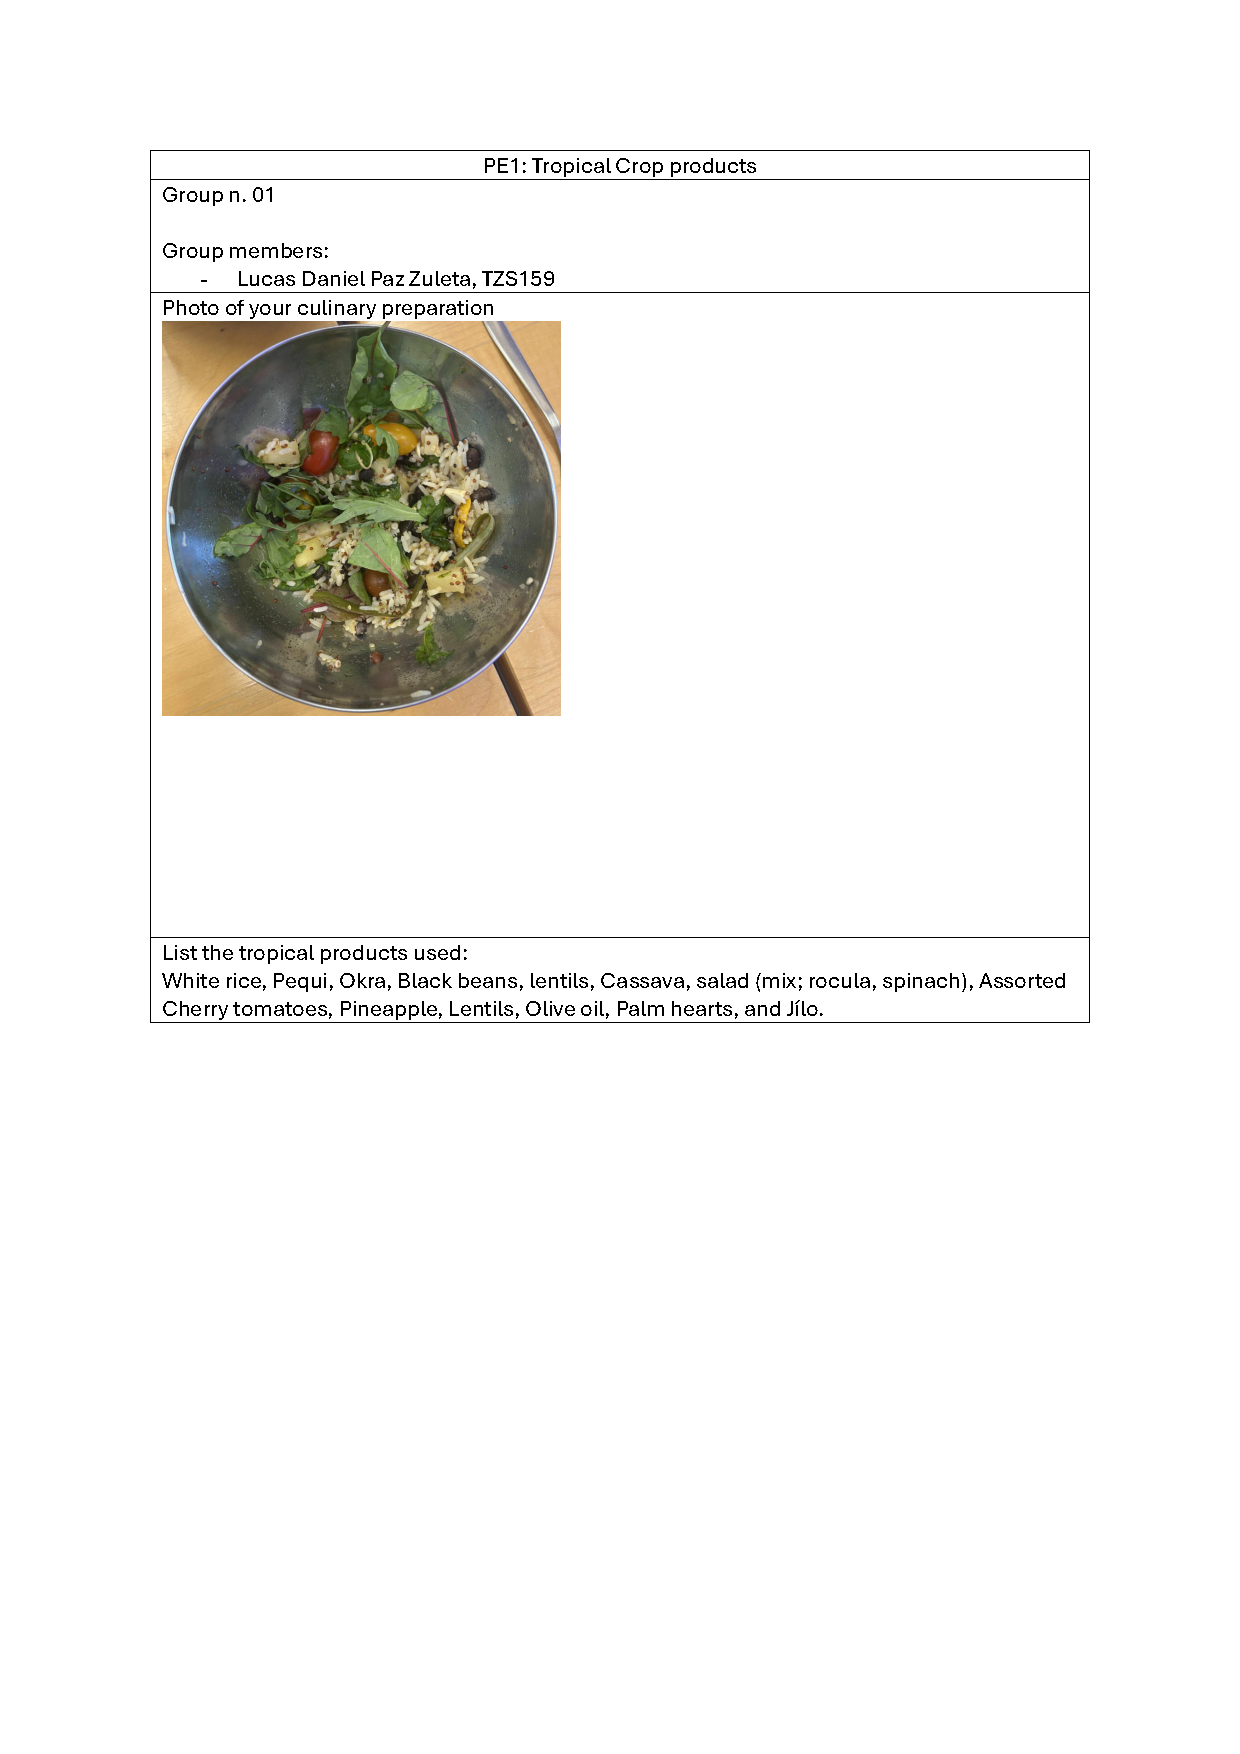
\includepdf[pages=-, scale=1]{Appendices/PE1.pdf}[H]



\end{appendices}

\end{document}